\section{Risultati}\label{risultati}

\subsection{Tabella con MST calcolati}
	
	\renewcommand{\arraystretch}{1.5}
	\begin{longtable}{|c|c|c|c|}
		\hline
		\rowcolor{title_row}
		\textbf{\color{title_text}{Input file}} &
		\textbf{\color{title_text}{num\_vertici}} & \textbf{\color{title_text}{num\_archi}} & \textbf{\color{title_text}{MST}}\\
		\hline
		\endhead
		input\_random\_01\_10.txt & 10 & 9 & 29316 \\ \hline 
		input\_random\_02\_10.txt & 10 & 13 & 2126 \\ \hline 
		input\_random\_03\_10.txt & 10 & 14 & -44765 \\ \hline
		input\_random\_04\_10.txt & 10 & 11 & 20360 \\ \hline
		input\_random\_05\_20.txt & 20 & 25 & -32021 \\ \hline
		input\_random\_06\_20.txt & 20 & 25 & 18596 \\ \hline
		input\_random\_07\_20.txt & 20 & 29 & -42560 \\ \hline
		input\_random\_08\_20.txt & 20 & 26 & -37205 \\ \hline
		input\_random\_09\_40.txt & 40 & 57 & -122078 \\ \hline
		input\_random\_10\_40.txt & 40 & 51 & -37021 \\ \hline
		input\_random\_11\_40.txt & 40 & 50 & -79570 \\ \hline
		input\_random\_12\_40.txt & 40 & 52 & -79741 \\ \hline
		input\_random\_13\_80.txt & 80 & 108 & -139926 \\ \hline
		input\_random\_14\_80.txt & 80 & 101 & -211345 \\ \hline
		input\_random\_15\_80.txt & 80 & 104 & -110571 \\ \hline
		input\_random\_16\_80.txt & 80 & 115 & -233320 \\ \hline
		input\_random\_17\_100.txt & 100 & 137 & -141960 \\ \hline
		input\_random\_18\_100.txt & 100 & 129 & -271743 \\ \hline
		input\_random\_19\_100.txt & 100 & 137 & -288906 \\ \hline
		input\_random\_20\_100.txt & 100 & 133 & -232178 \\ \hline
		input\_random\_21\_200.txt & 200 & 268 & -510185 \\ \hline
		input\_random\_22\_200.txt & 200 & 269 & -515136 \\ \hline
		input\_random\_23\_200.txt & 200 & 269 & -444357 \\ \hline
		input\_random\_24\_200.txt & 200 & 267 & -393278 \\ \hline
		input\_random\_25\_400.txt & 400 & 541 & -1122919 \\ \hline
		input\_random\_26\_400.txt & 400 & 518 & -788168 \\ \hline
		input\_random\_27\_400.txt & 400 & 539 & -895704 \\ \hline
		input\_random\_28\_400.txt & 400 & 526 & -733645 \\ \hline
		input\_random\_29\_800.txt & 800 & 1026 & -1541291 \\ \hline
		input\_random\_30\_800.txt & 800 & 1059 & -1578294 \\ \hline
		input\_random\_31\_800.txt & 800 & 1078 & -1675534 \\ \hline
		input\_random\_32\_800.txt & 800 & 1050 & -1652119 \\ \hline
		input\_random\_33\_1000.txt & 1000 & 1301 & -2091110 \\ \hline
		input\_random\_34\_1000.txt & 1000 & 1313 & -1934208 \\ \hline
		input\_random\_35\_1000.txt & 1000 & 1328 & -2229428 \\ \hline
		input\_random\_36\_1000.txt & 1000 & 1345 & -2359192 \\ \hline
		input\_random\_37\_2000.txt & 2000 & 2699 & -4811598 \\ \hline
		input\_random\_38\_2000.txt & 2000 & 2654 & -4739387 \\ \hline
		input\_random\_39\_2000.txt & 2000 & 2652 & -4717250 \\ \hline
		input\_random\_40\_2000.txt & 2000 & 2677 & -4537267 \\ \hline
		input\_random\_41\_4000.txt & 4000 & 5361 & -8722212 \\ \hline
		input\_random\_42\_4000.txt & 4000 & 5316 & -9314968 \\ \hline
		input\_random\_43\_4000.txt & 4000 & 5340 & -9845767 \\ \hline
		input\_random\_44\_4000.txt & 4000 & 5369 & -8681447 \\ \hline
		input\_random\_45\_8000.txt & 8000 & 10706 & -17844628 \\ \hline
		input\_random\_46\_8000.txt & 8000 & 10672 & -18800966 \\ \hline
		input\_random\_47\_8000.txt & 8000 & 10662 & -18741474 \\ \hline
		input\_random\_48\_8000.txt & 8000 & 10758 & -18190442 \\ \hline
		input\_random\_49\_10000.txt & 10000 & 13302 & -22086729 \\ \hline
		input\_random\_50\_10000.txt & 10000 & 13342 & -22338561 \\ \hline
		input\_random\_51\_10000.txt & 10000 & 13287 & -22581384 \\ \hline
		input\_random\_52\_10000.txt & 10000 & 13287 & -22606313 \\ \hline
		input\_random\_53\_20000.txt & 20000 & 26671 & -45978687 \\ \hline
		input\_random\_54\_20000.txt & 20000 & 26826 & -45195405 \\ \hline
		input\_random\_55\_20000.txt & 20000 & 26674 & -47854708 \\ \hline
		input\_random\_56\_20000.txt & 20000 & 26671 & -46420311 \\ \hline
		input\_random\_57\_40000.txt & 40000 & 53415 & -92003321 \\ \hline
		input\_random\_58\_40000.txt & 40000 & 53447 & -94397064 \\ \hline
		input\_random\_59\_40000.txt & 40000 & 53243 & -88783643 \\ \hline
		input\_random\_60\_40000.txt & 40000 & 53319 & -93017025 \\ \hline
		input\_random\_61\_80000.txt & 80000 & 106587 & -186834082 \\ \hline
		input\_random\_62\_80000.txt & 80000 & 106634 & -185997521 \\ \hline
		input\_random\_63\_80000.txt & 80000 & 106587 & -182065015 \\ \hline
		input\_random\_64\_80000.txt & 80000 & 106555 & -180803872 \\ \hline
		input\_random\_65\_100000.txt & 100000 & 133395 & -230698391 \\ \hline
		input\_random\_66\_100000.txt & 100000 & 133214 & -230168572 \\ \hline
		input\_random\_67\_100000.txt & 100000 & 133525 & -231393935 \\ \hline
		input\_random\_68\_100000.txt & 100000 & 133463 & -231011693 \\ \hline
	\end{longtable}

\subsection{Grafico delle performance dell'algoritmo di Prim}

	\begin{centering}
		\begin{figure}[H]
			\hspace{-1cm}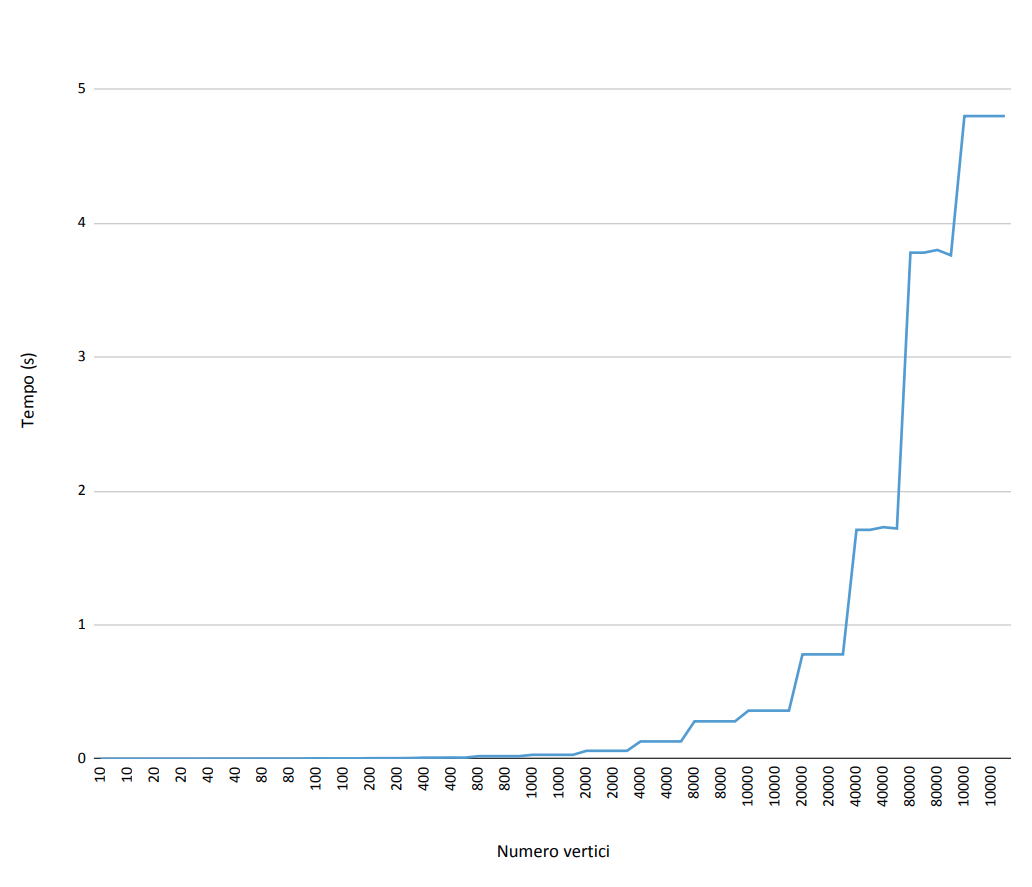
\includegraphics[width=19cm]{Img/prim_result.png}
			\caption{Performance dell'algoritmo di Prim}
		\end{figure}
	\end{centering}

\subsection{Grafico delle performance dell'algoritmo di Kruskal ``naive''}
	\begin{figure}[H]
		\hspace{-1cm}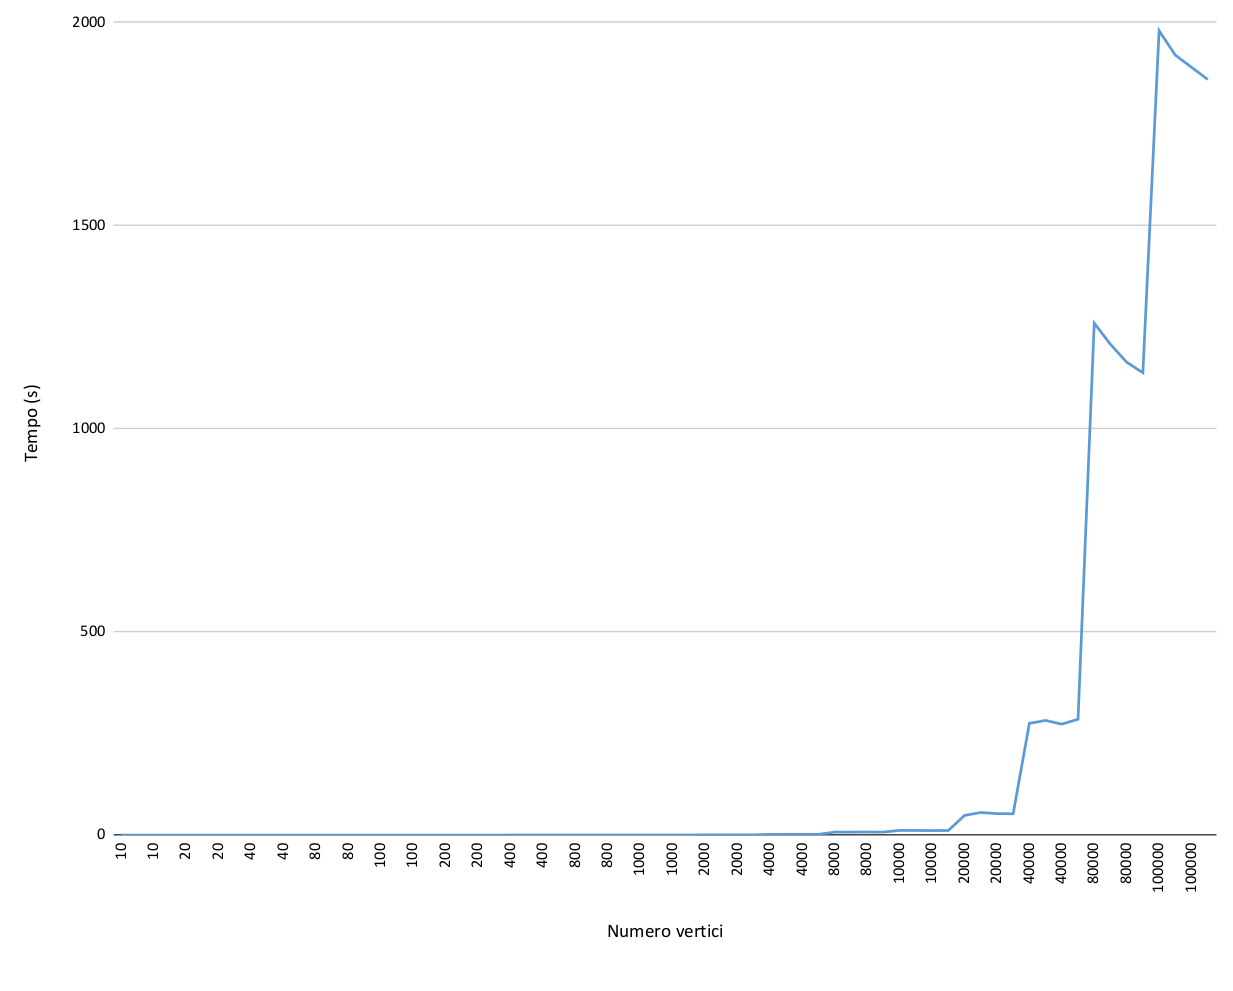
\includegraphics[width=18.5cm]{Img/kruskal_naive_result.png}
		\caption{Performance dell'algoritmo di Kruskal ``naive''}
	\end{figure}

\subsection{Grafico delle performance dell'algoritmo di Kruskal Union Find}
	\begin{figure}[H]
	 	\hspace{-1cm}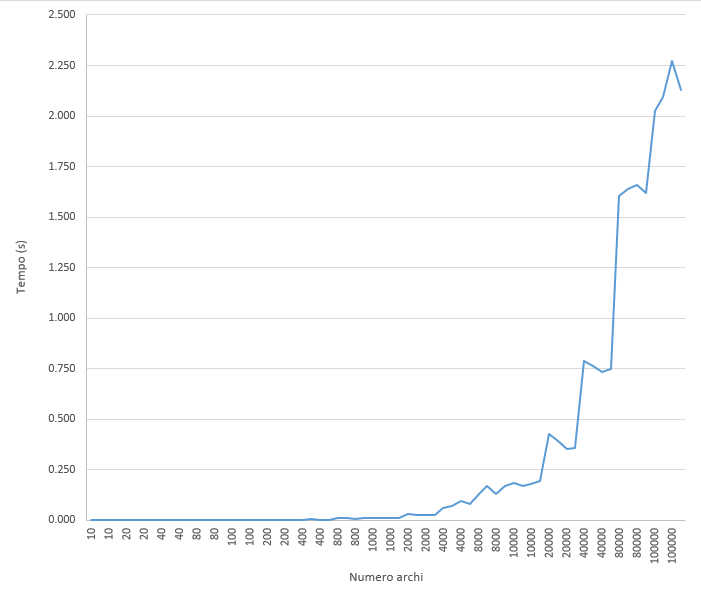
\includegraphics[width=18.5cm]{Img/kruskal_uf_result.png}
		\caption{Performance dell'algoritmo di Kruskal con Union Find}
	\end{figure}


\pagebreak